En este capítulo, se detalla el plan para implementar y poner en funcionamiento el software del brazo robótico.
\section{Plan de implantación}

La aplicación se ha concebido con la premisa de ser accesible, por lo tanto:
\begin{enumerate}
    \item Se debe descargar.
    \item Se debe descomprimir.
    \item Utilizar.
\end{enumerate}

La aparente simplicidad de esta plataforma se encuentra intrínsecamente vinculada a su principal propósito: facilitar a los estudiantes la ejecución de operaciones en los equipos del laboratorio, prescindiendo de la necesidad de su presencia física. Este enfoque, busca proporcionar una experiencia de aprendizaje remoto que permita a los participantes interactuar con los recursos de manera eficaz y sin complicaciones, garantizando así un acceso fluido a las herramientas de laboratorio desde cualquier ubicación geográfica.

A continuación, se presenta un análisis de las instrucciones para la utilización de esta plataforma. Las indicaciones, abarcan aspectos clave que orientan a los usuarios en para poder acceder a la aplicación.

\clearpage
\section*{Instrucciones para el uso}

\subsection*{Descarga de la Aplicación}
Este paso es común para todos los sistemas, usando el navegador de internet de preferencia, se debe acceder al repositorio de GitHub \footnote{\url{https://github.com/Patricio1Labra/SimuladorCIMUBB}}
\begin{enumerate}[label=\arabic*.-]
    
\begin{figure}[ht]
    \centering
    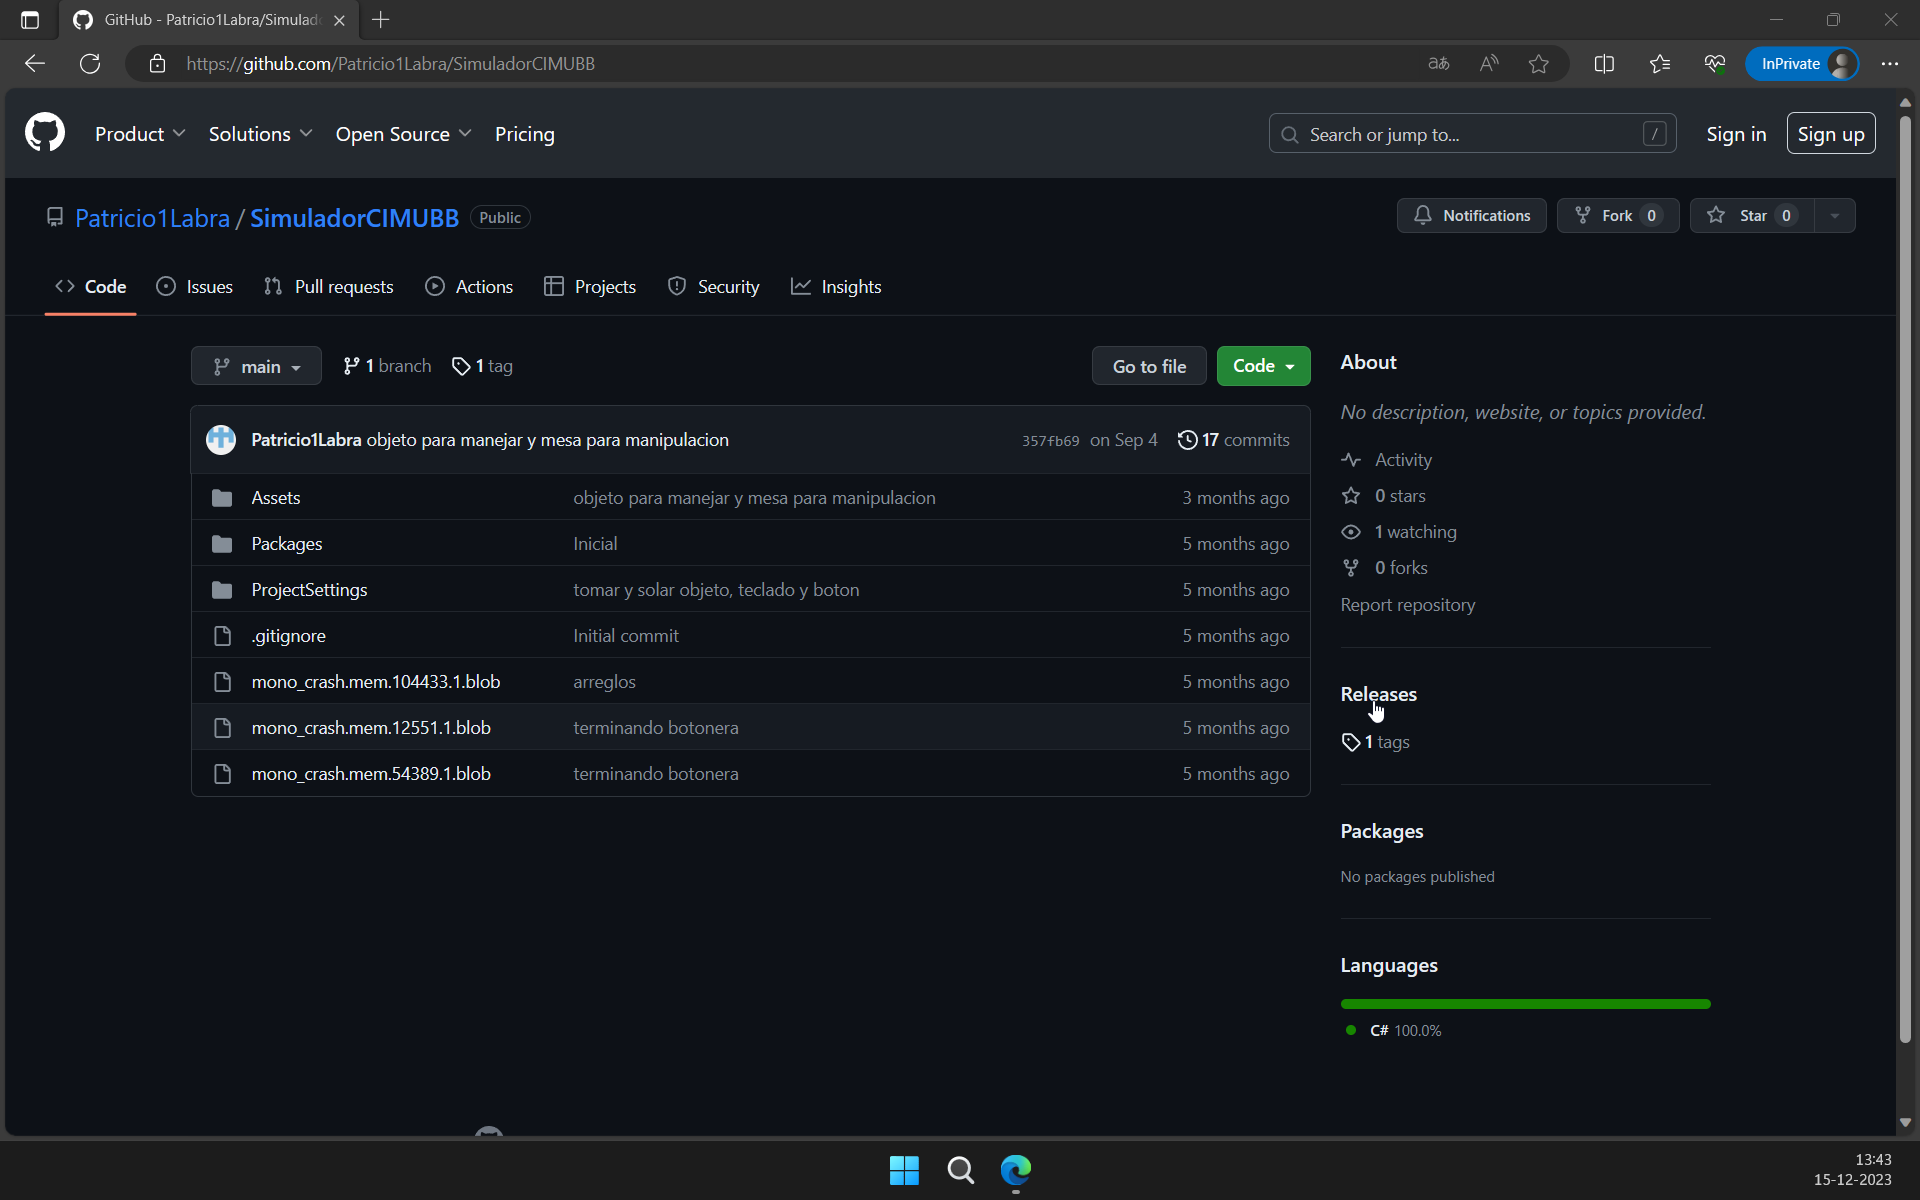
\includegraphics[width=13cm]{figures/TutorialWindows/tutorial (1).png}
    \caption{Parte 1 Tutorial}
    \label{fig:tutowin1}
\end{figure}
    \item 

\begin{figure}[ht]
    \centering
    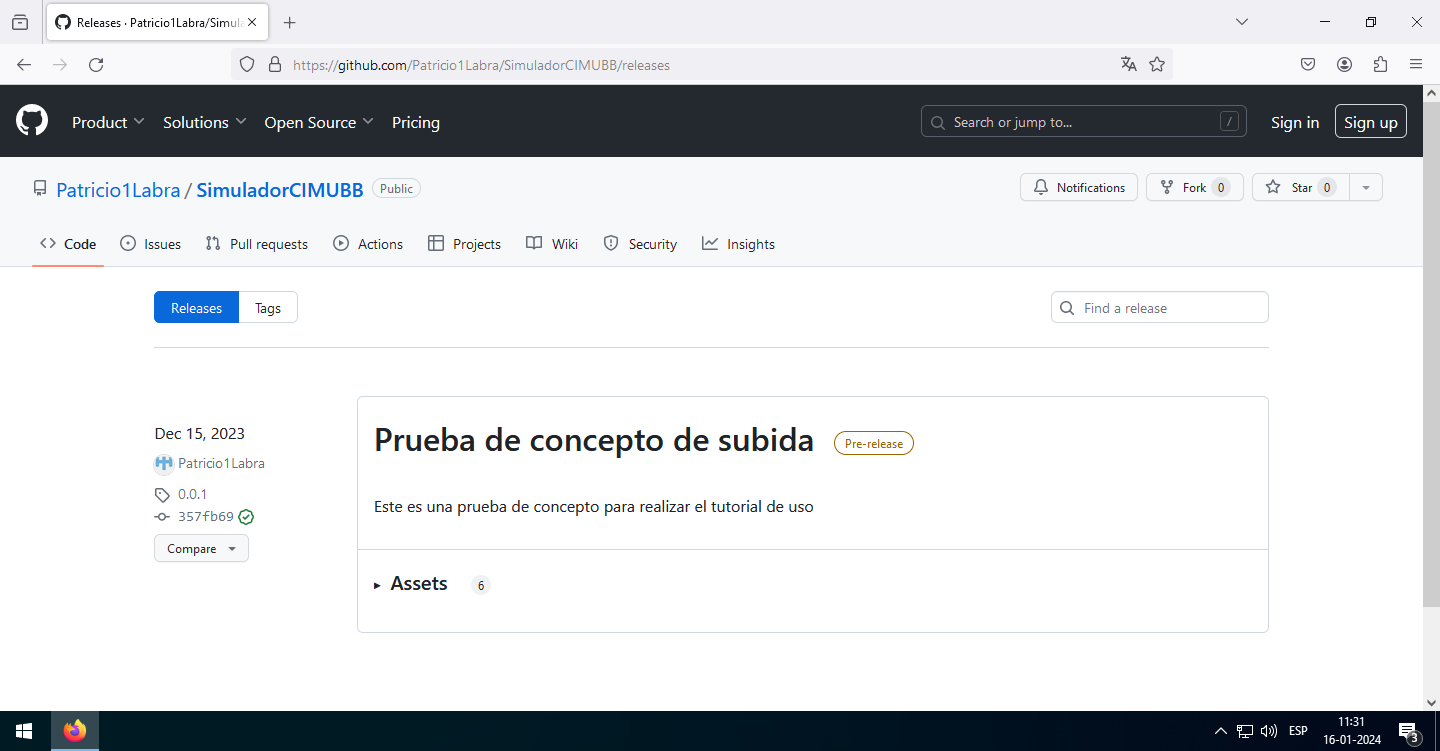
\includegraphics[width=13cm]{figures/TutorialWindows/tutorial (2).png}
    \caption{Parte 2 Tutorial}
    \label{fig:tutowin2}
\end{figure}

\begin{figure}[ht]
    \centering
    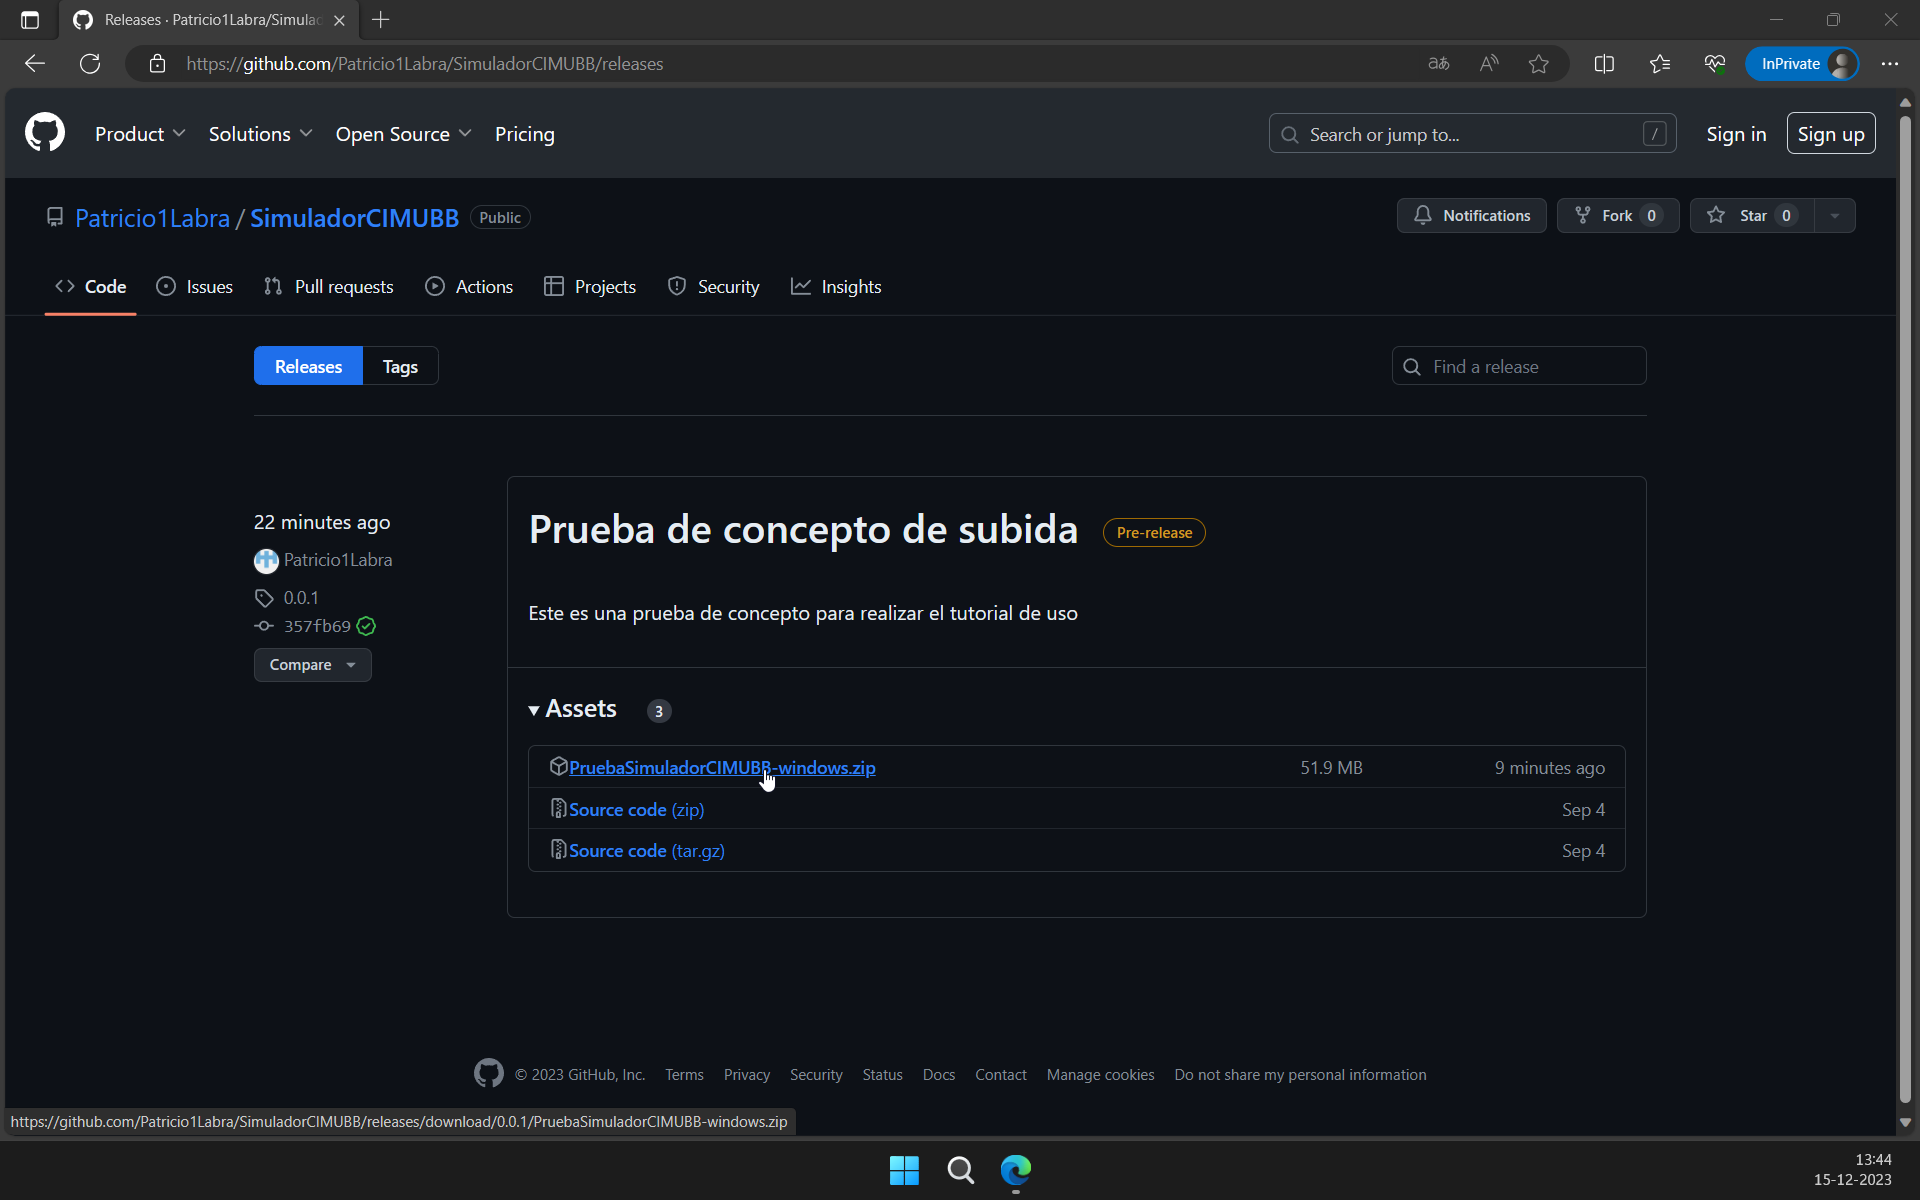
\includegraphics[width=13cm]{figures/TutorialWindows/tutorial (3).png}
    \caption{Parte 3 Tutorial}
    \label{fig:tutowin3}
\end{figure}

\begin{figure}[ht]
    \centering
    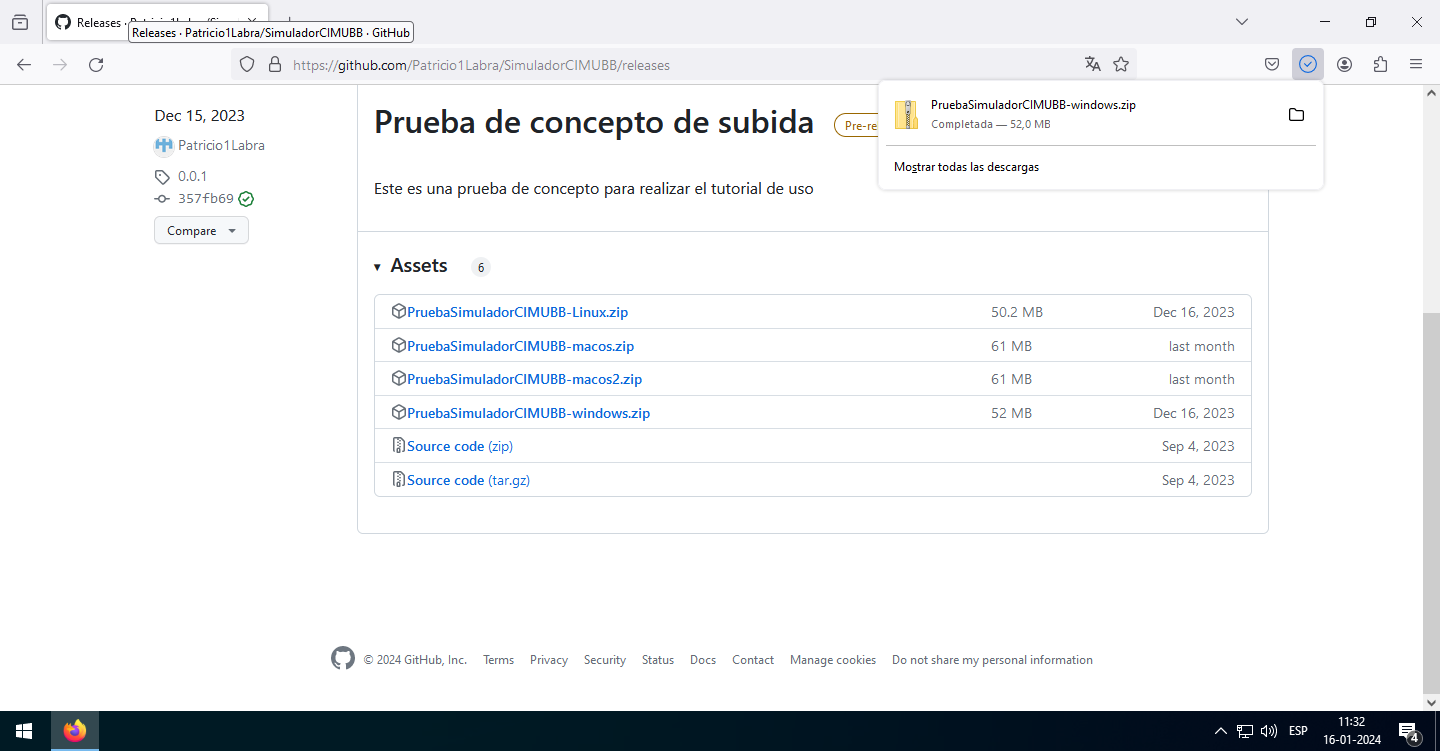
\includegraphics[width=13cm]{figures/TutorialWindows/tutorial (4).png}
    \caption{Parte 4 Tutorial}
    \label{fig:tutowin4}
\end{figure}

\begin{figure}[ht]
    \centering
    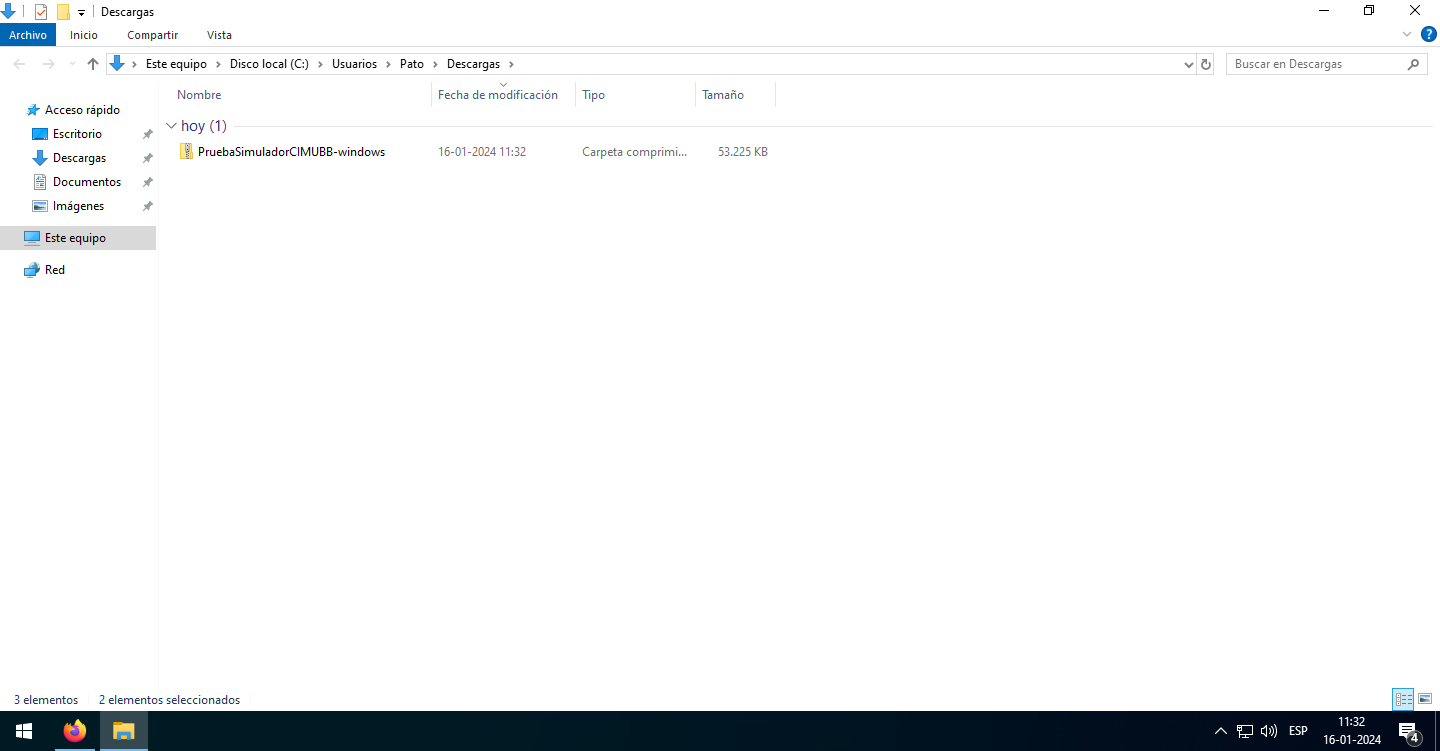
\includegraphics[width=13cm]{figures/TutorialWindows/tutorial (5).png}
    \caption{Parte 5 Tutorial}
    \label{fig:tutowin5}
\end{figure}
\end{enumerate}
\clearpage

\subsection*{Descomprimir}

\subsubsection*{Windows}

\begin{enumerate}[label=\arabic*.-]
    \item (Opcional) Descargar e instalar WinRAR u otro programa de su preferencia para descomprimir archivos ZIP. Solo si el sistema no le permite descomprimir el archivo nativamente.
    \begin{figure}[ht]
        \centering
        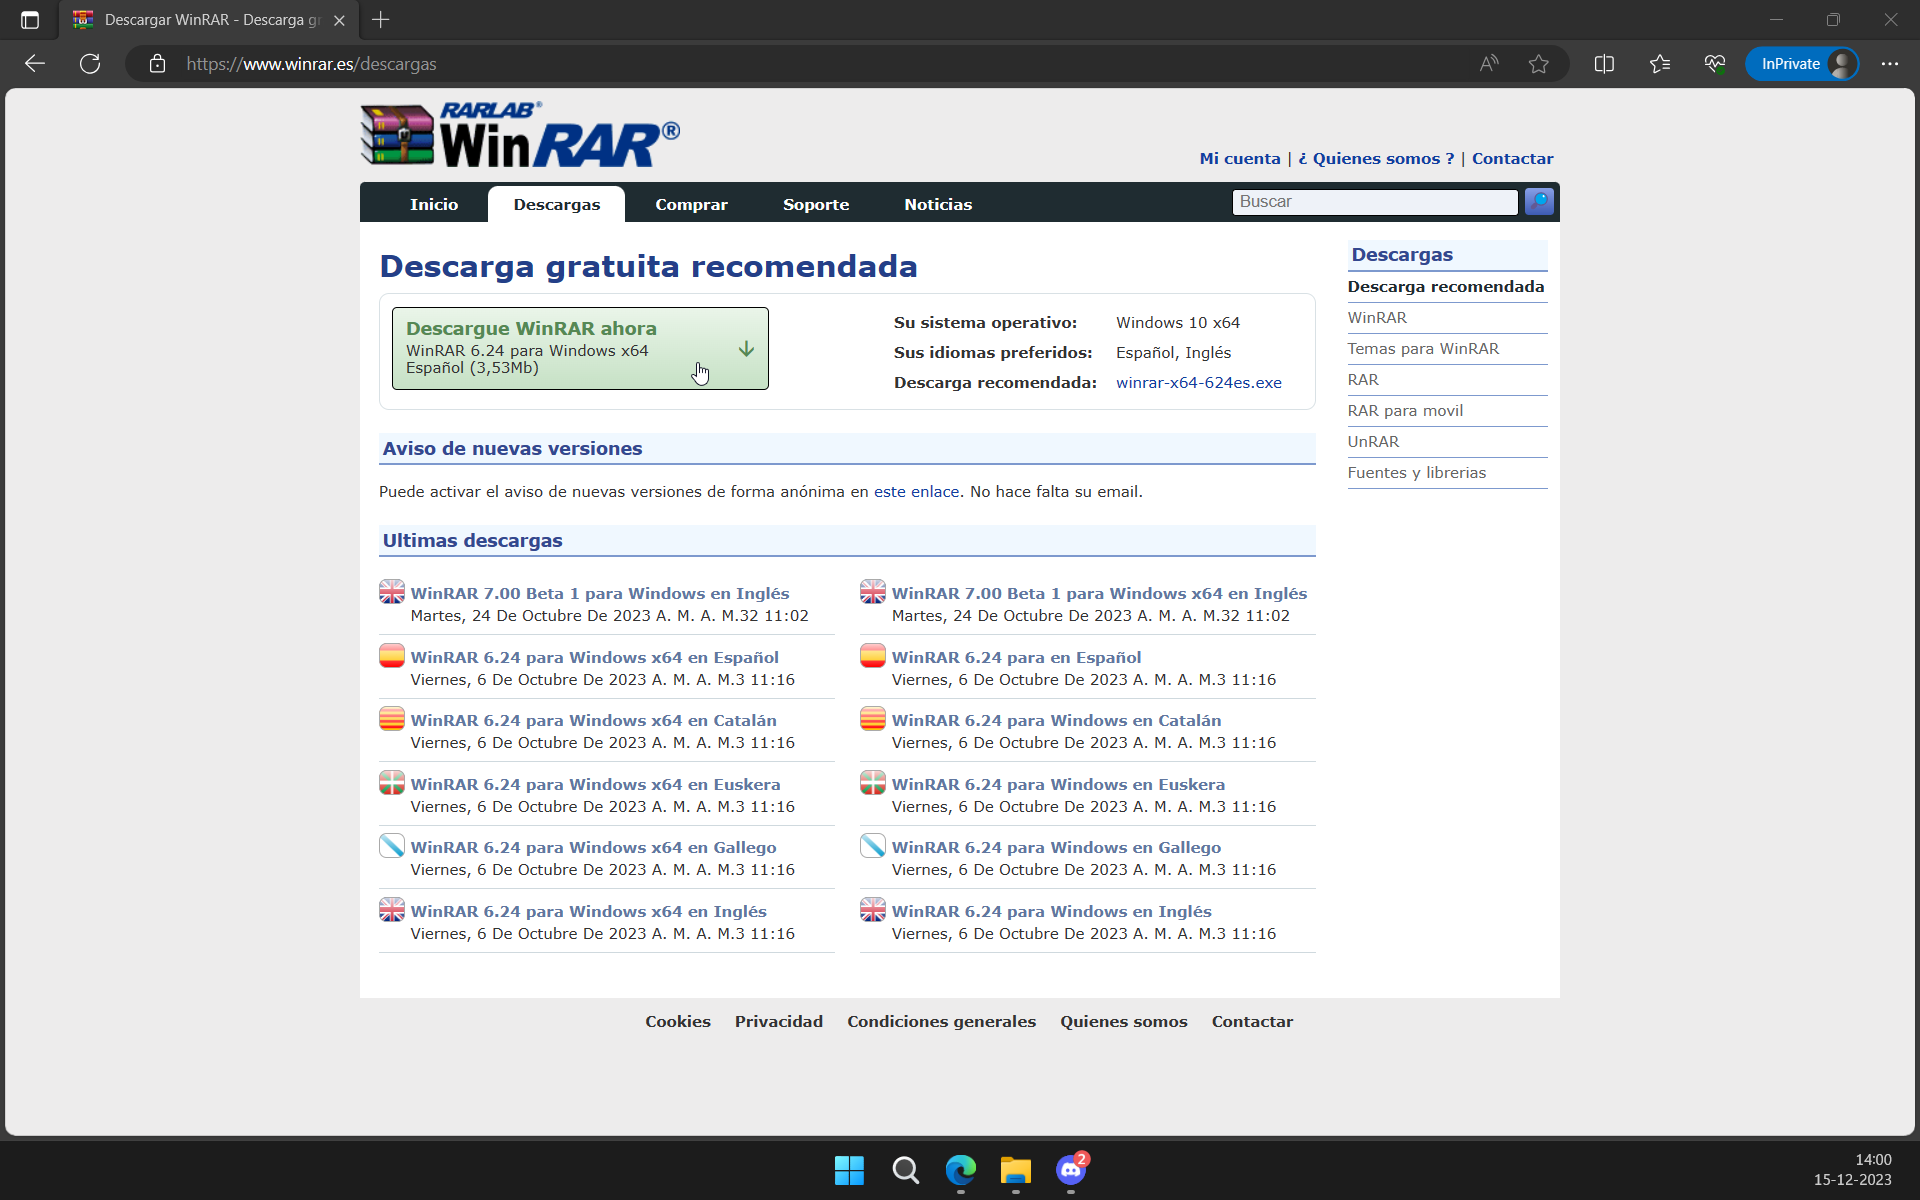
\includegraphics[width=13cm]{figures/TutorialWindows/winrar.png}
        \caption{Página de descarga WinRAR}
        \label{fig:winrar}
    \end{figure}
    \item Descargar el archivo ZIP desde GitHub.
    \item Descomprimir el archivo ZIP haciendo clic derecho y seleccionando ''Extraer aquí''.
\end{enumerate}

\begin{figure}[ht]
    \centering
    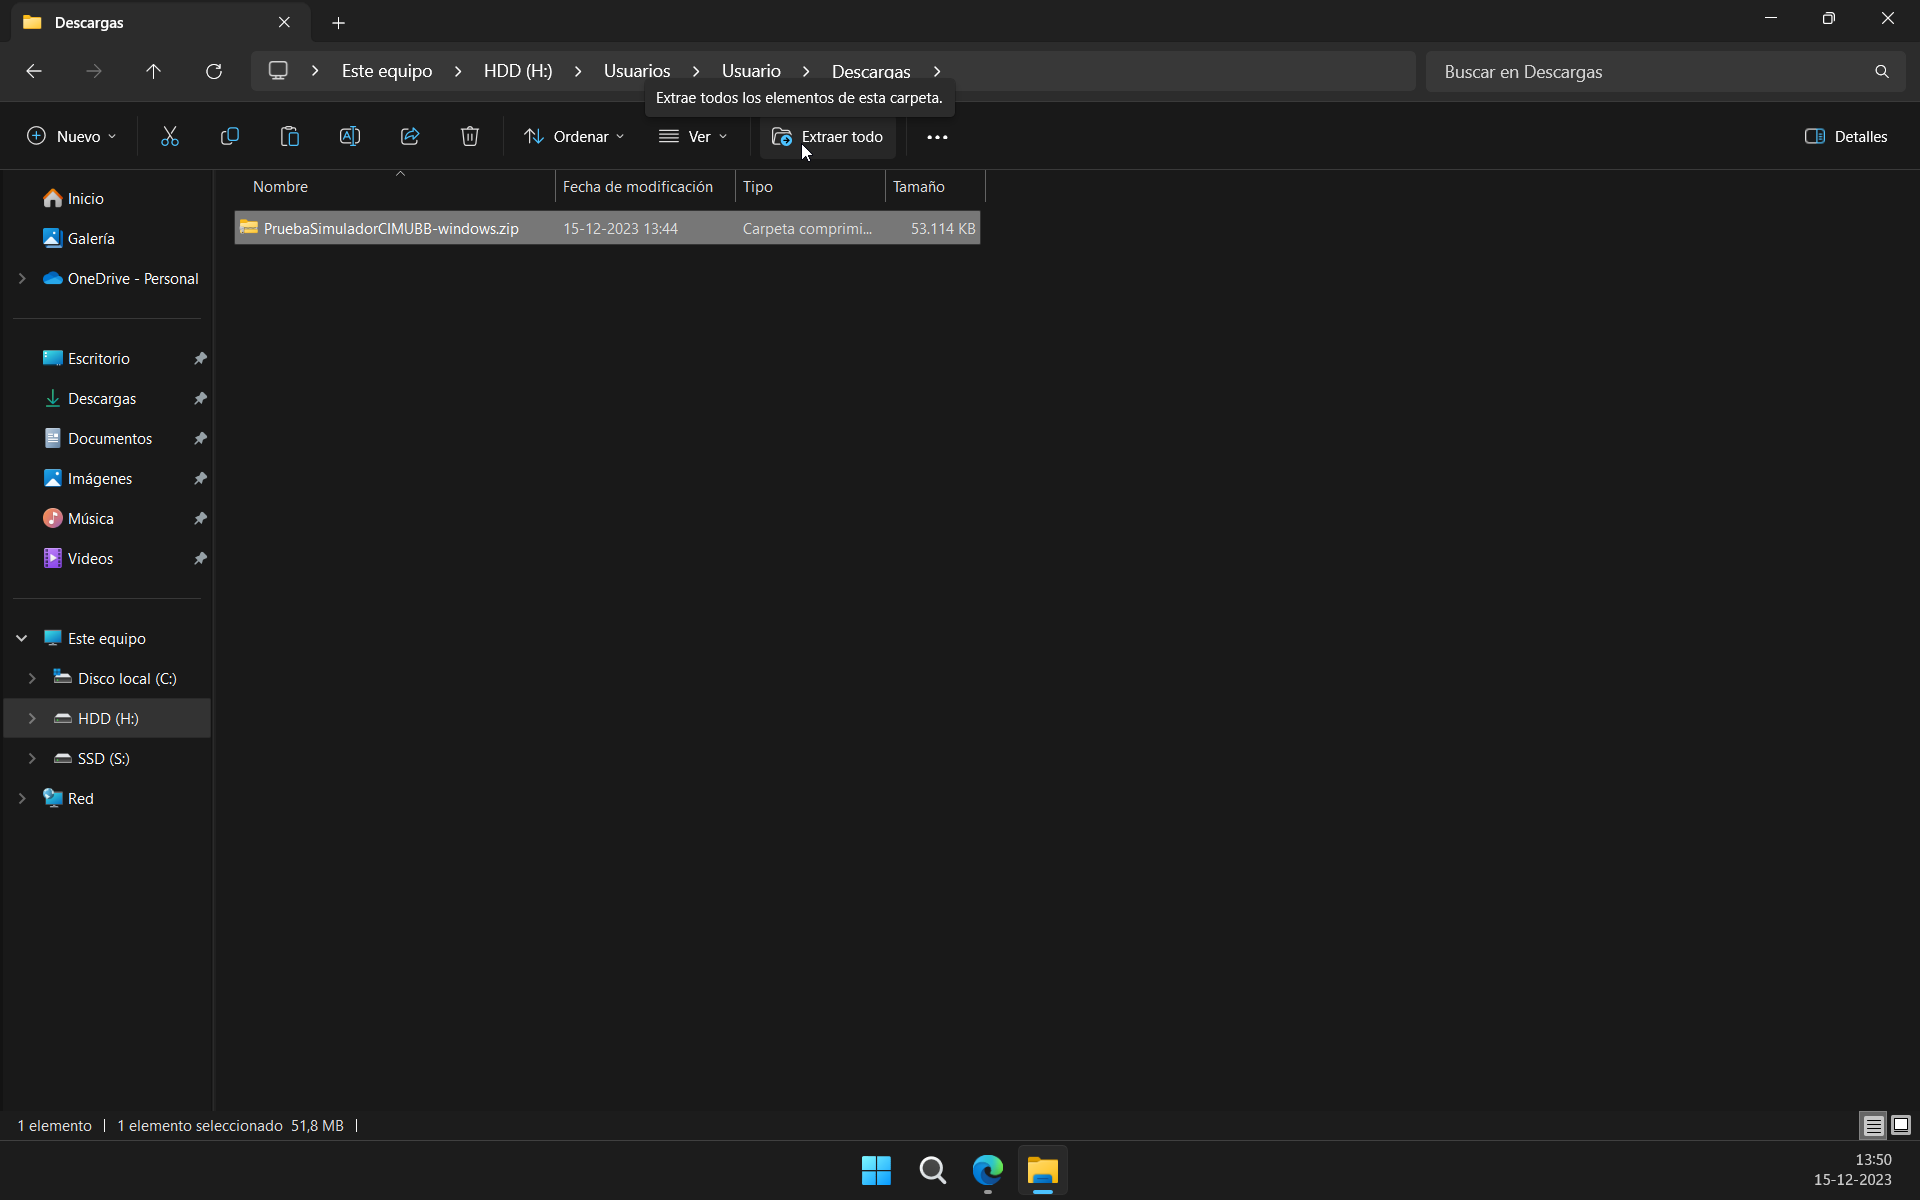
\includegraphics[width=13cm]{figures/TutorialWindows/tutorial (6).png}
    \caption{Parte 6 Tutorial Windows}
    \label{fig:tutowin6}
\end{figure}

\begin{figure}[ht]
    \centering
    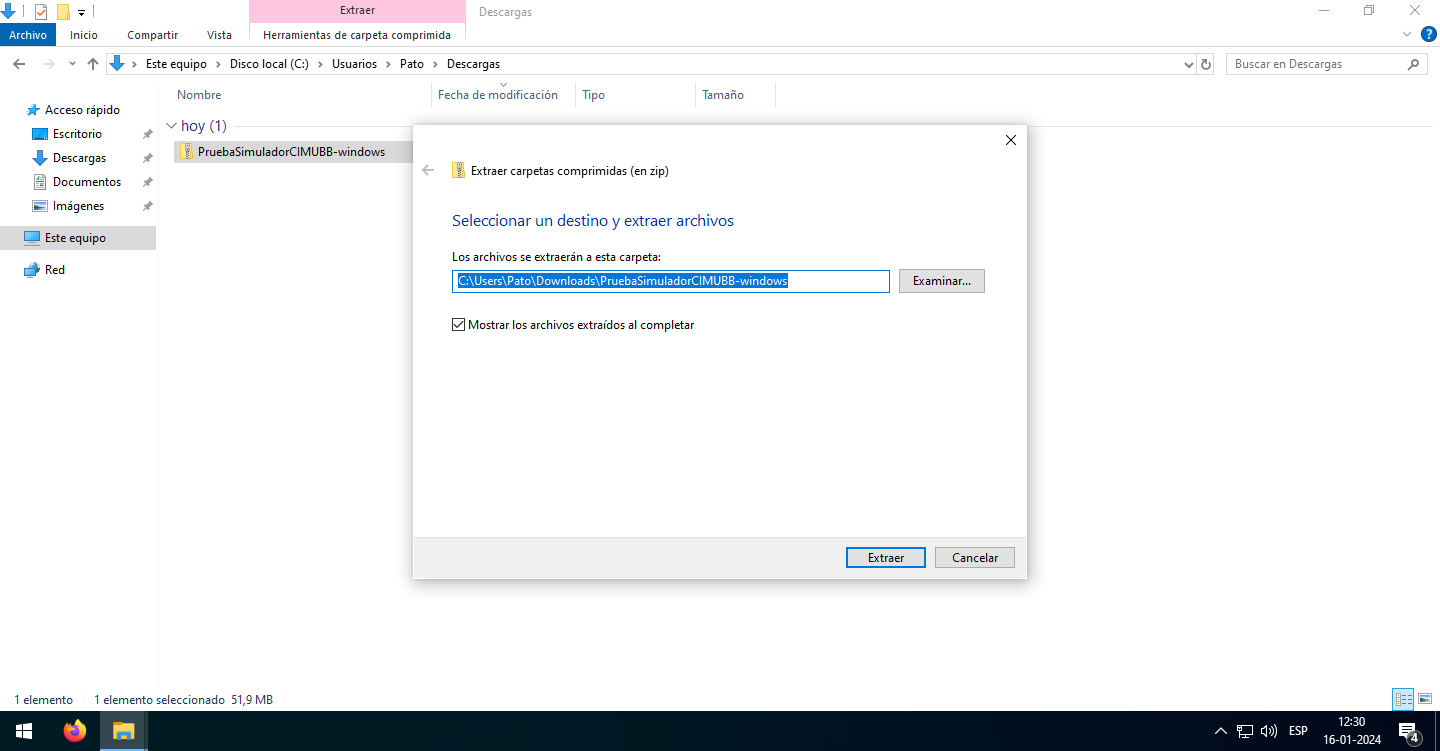
\includegraphics[width=13cm]{figures/TutorialWindows/tutorial (7).png}
    \caption{Parte 7 Tutorial Windows}
    \label{fig:tutowin7}
\end{figure}

\begin{figure}[ht]
    \centering
    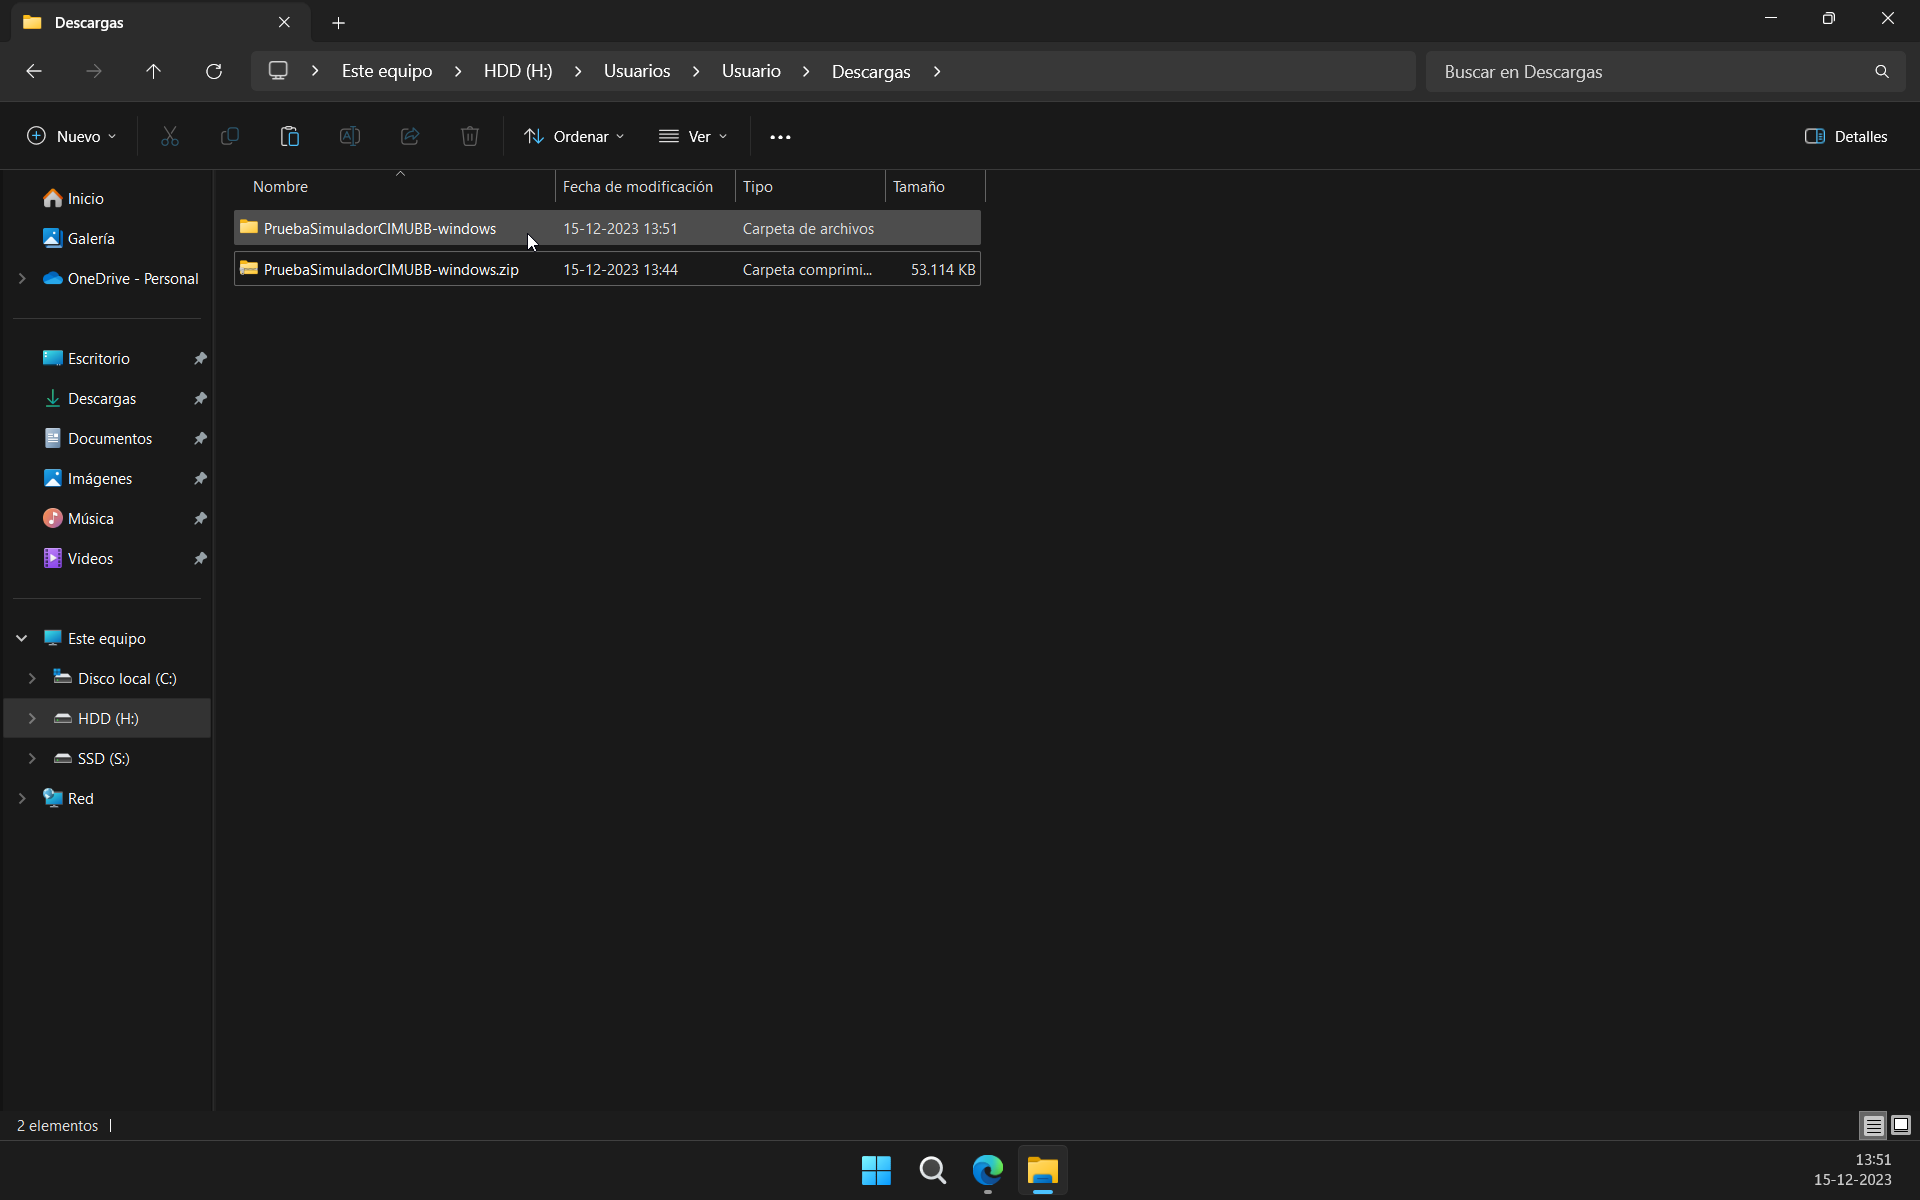
\includegraphics[width=13cm]{figures/TutorialWindows/tutorial (8).png}
    \caption{Parte 8 Tutorial Windows}
    \label{fig:tutowin8}
\end{figure}

\begin{figure}[ht]
    \centering
    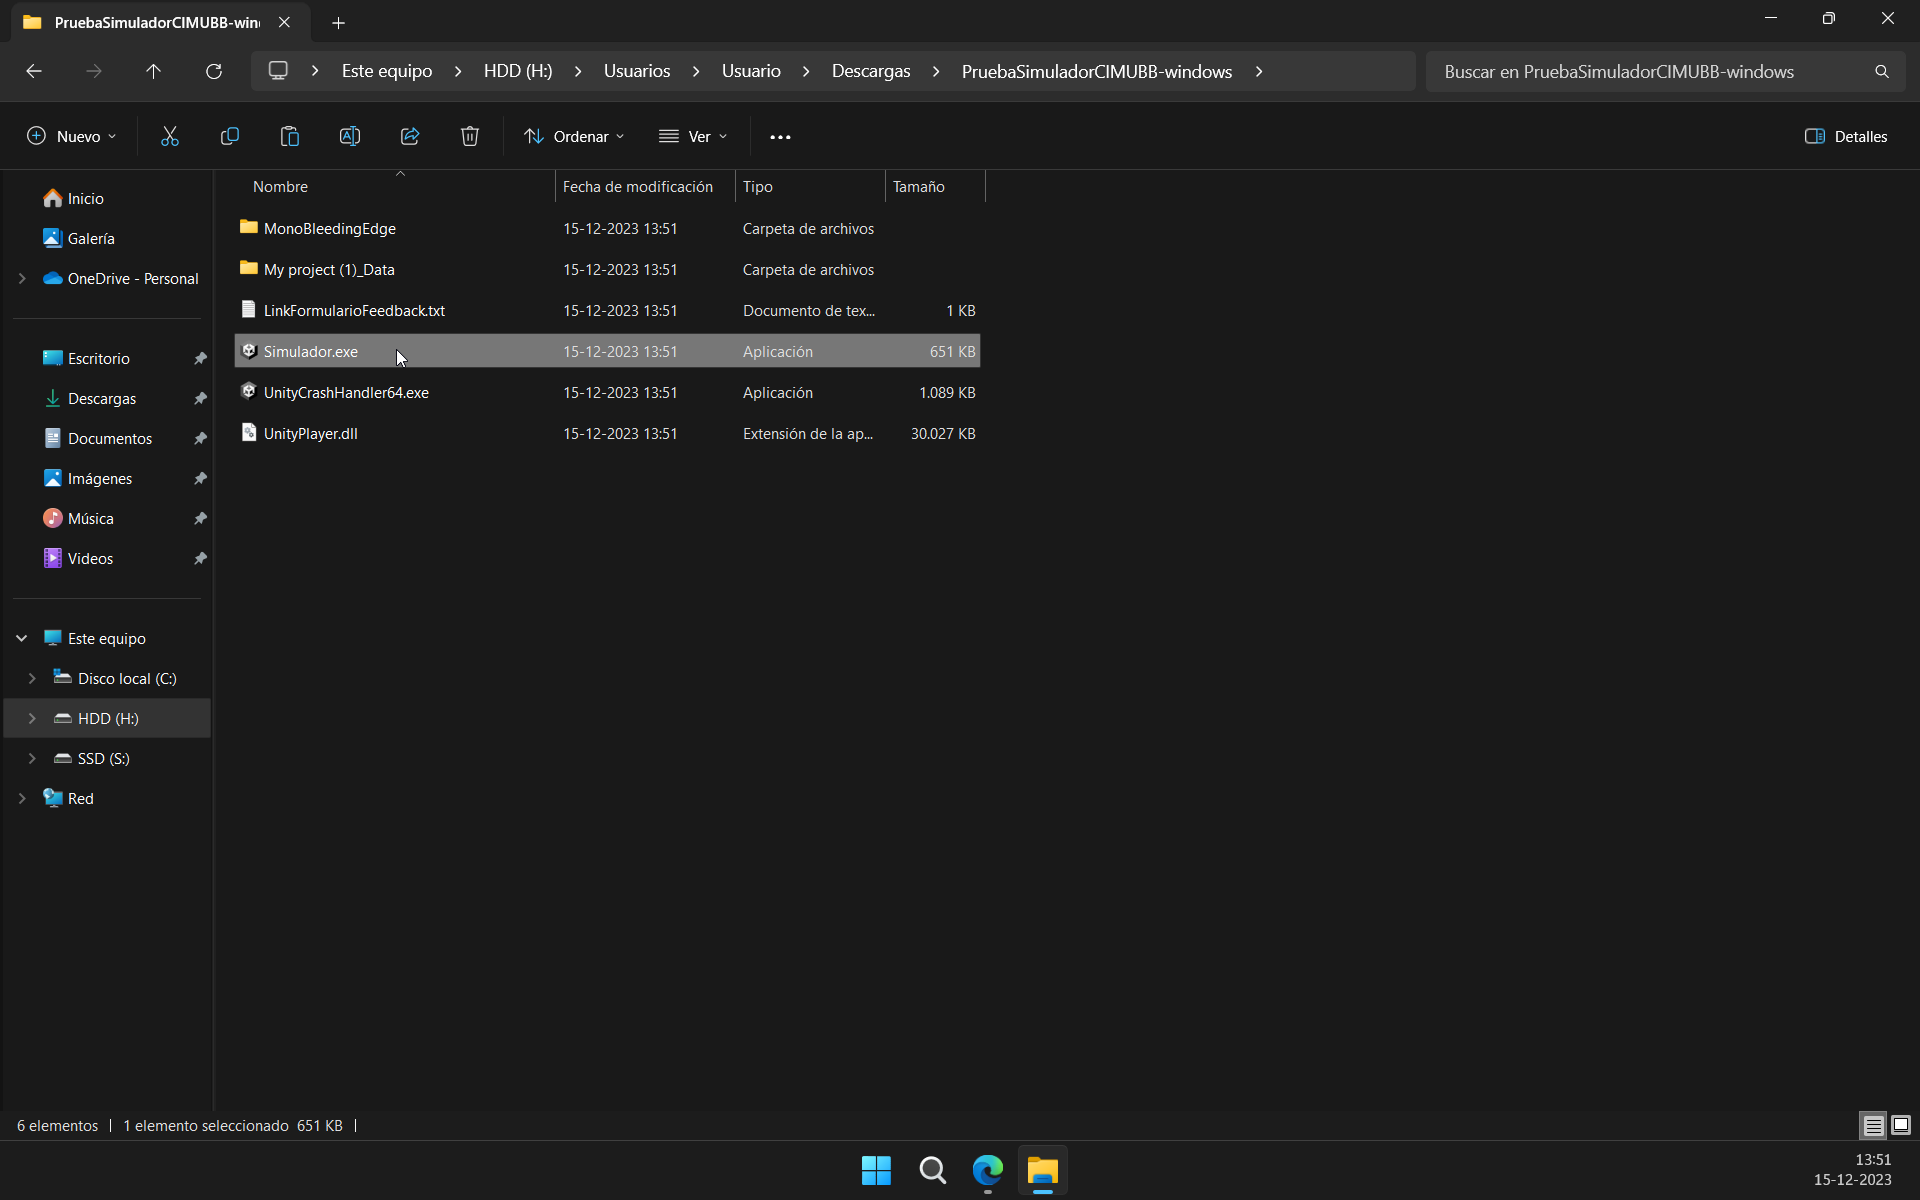
\includegraphics[width=13cm]{figures/TutorialWindows/tutorial (9).png}
    \caption{Parte 9 Tutorial Windows}
    \label{fig:tutowin9}
\end{figure}

\begin{figure}[ht]
    \centering
    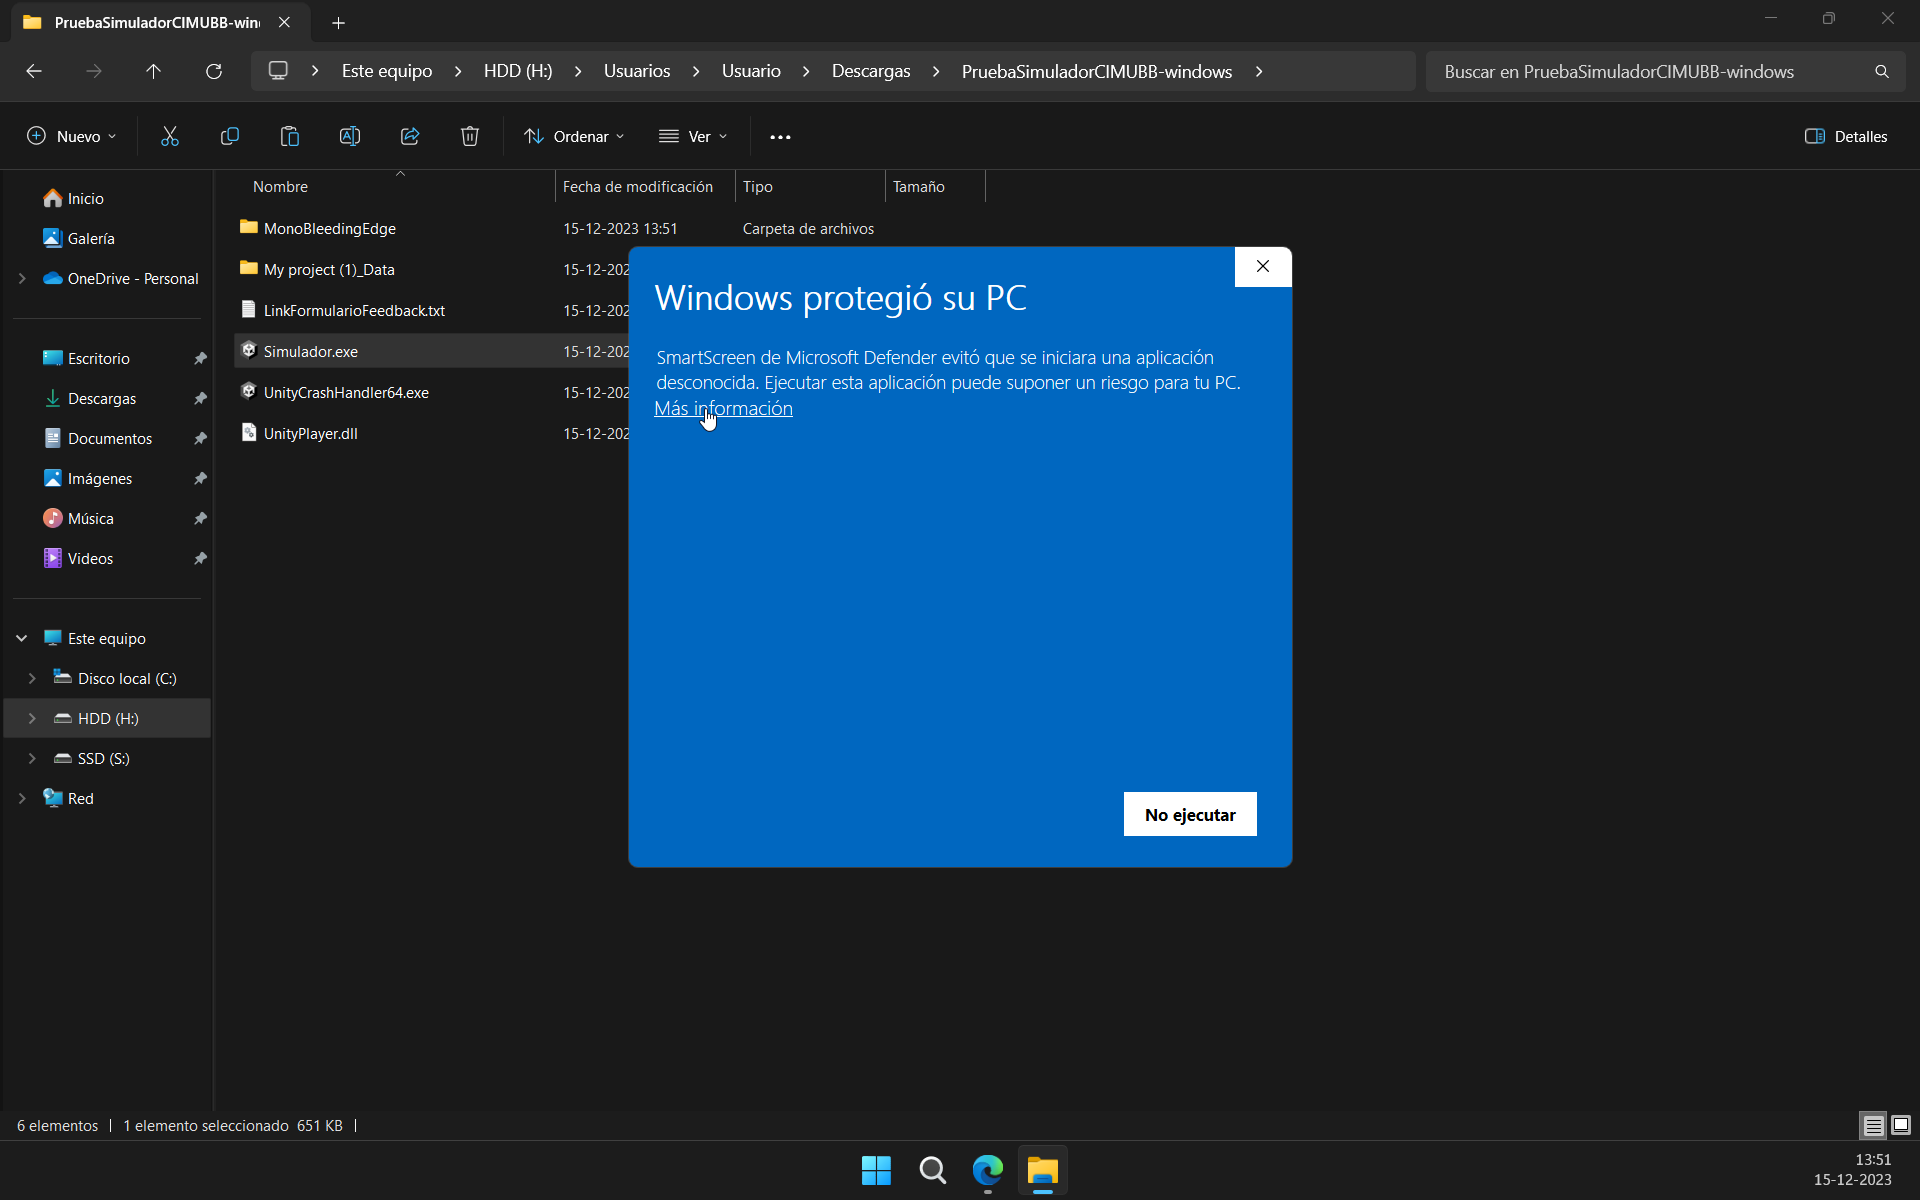
\includegraphics[width=13cm]{figures/TutorialWindows/tutorial (10).png}
    \caption{Parte 10 Tutorial Windows}
    \label{fig:tutowin10}
\end{figure}

\begin{figure}[ht]
    \centering
    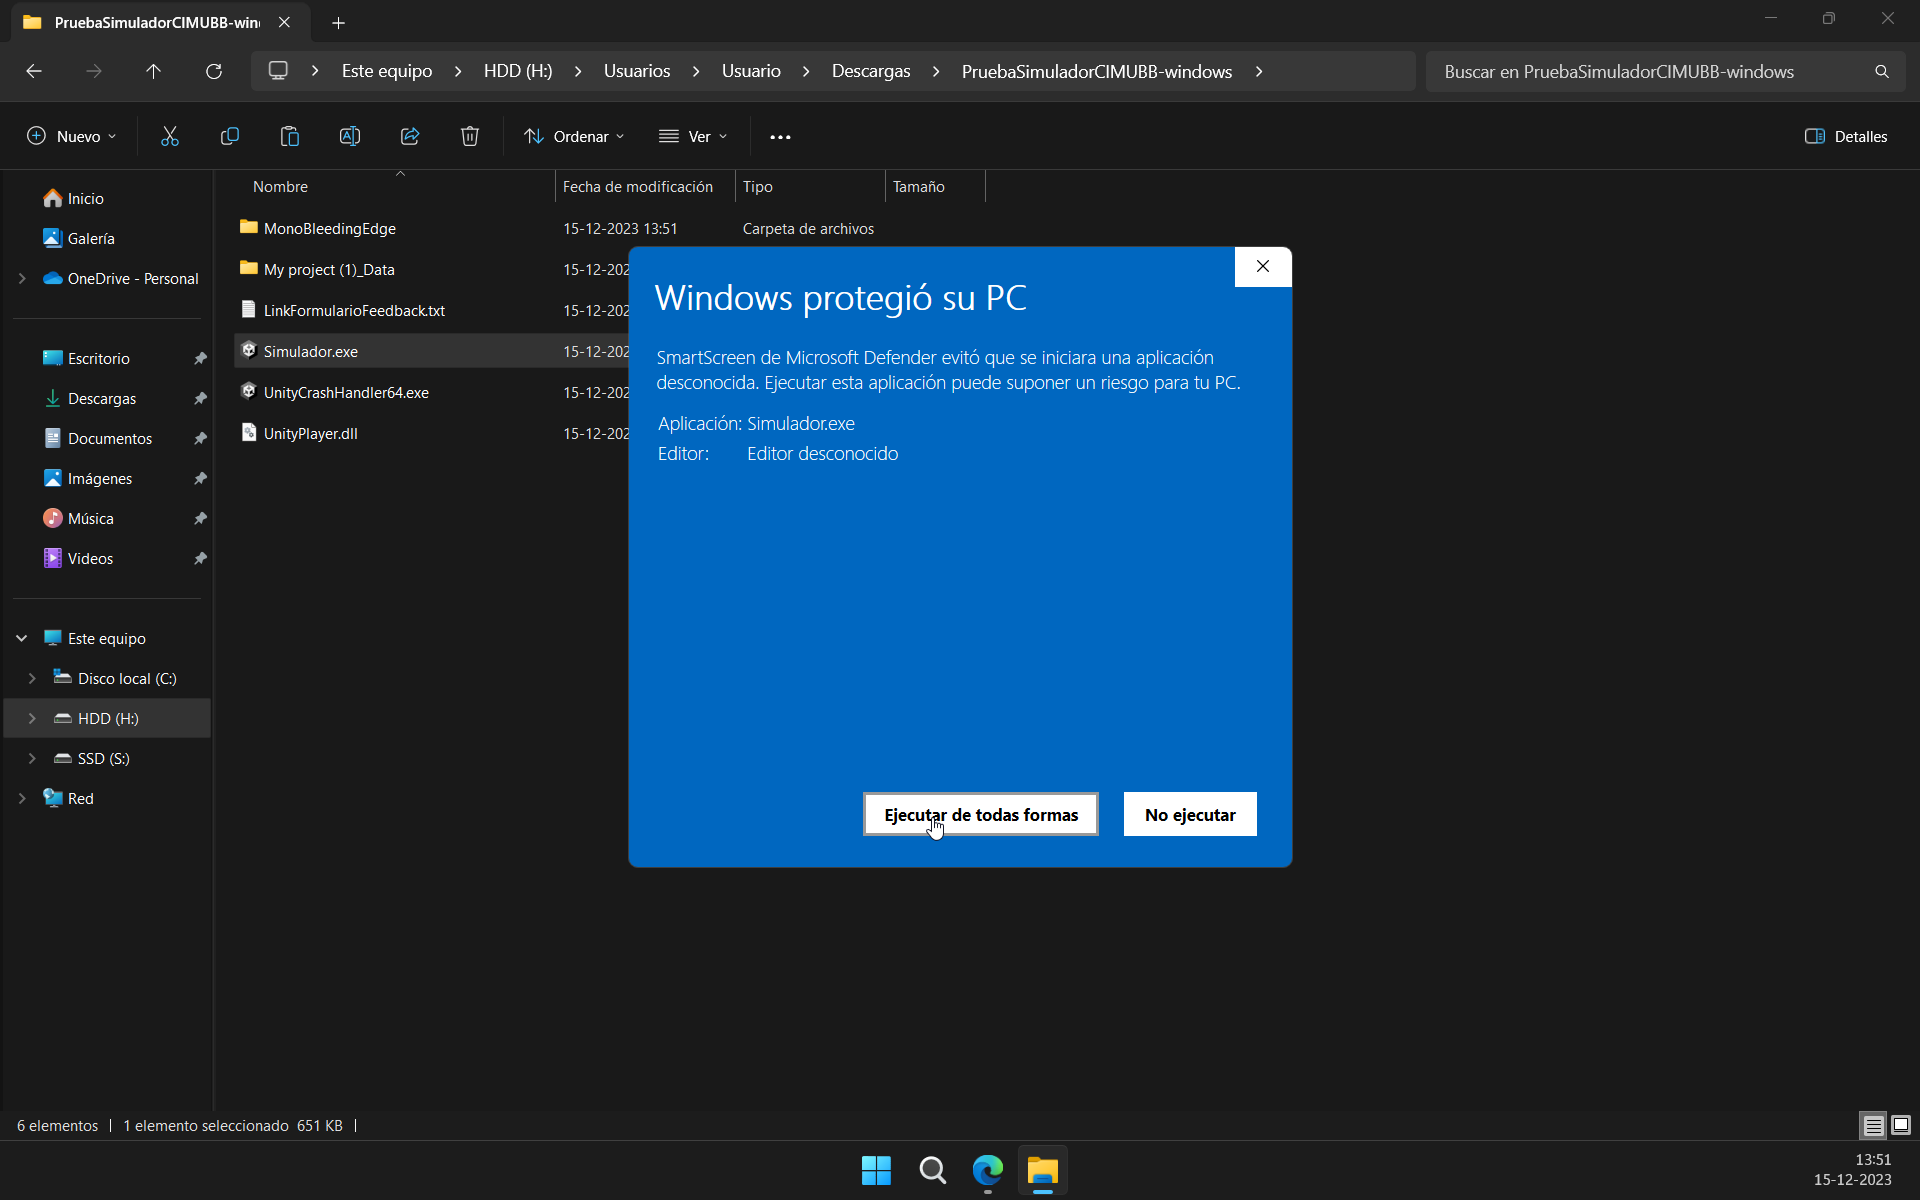
\includegraphics[width=13cm]{figures/TutorialWindows/tutorial (11).png}
    \caption{Parte 11 Tutorial Windows}
    \label{fig:tutowin11}
\end{figure}

\begin{figure}[ht]
    \centering
    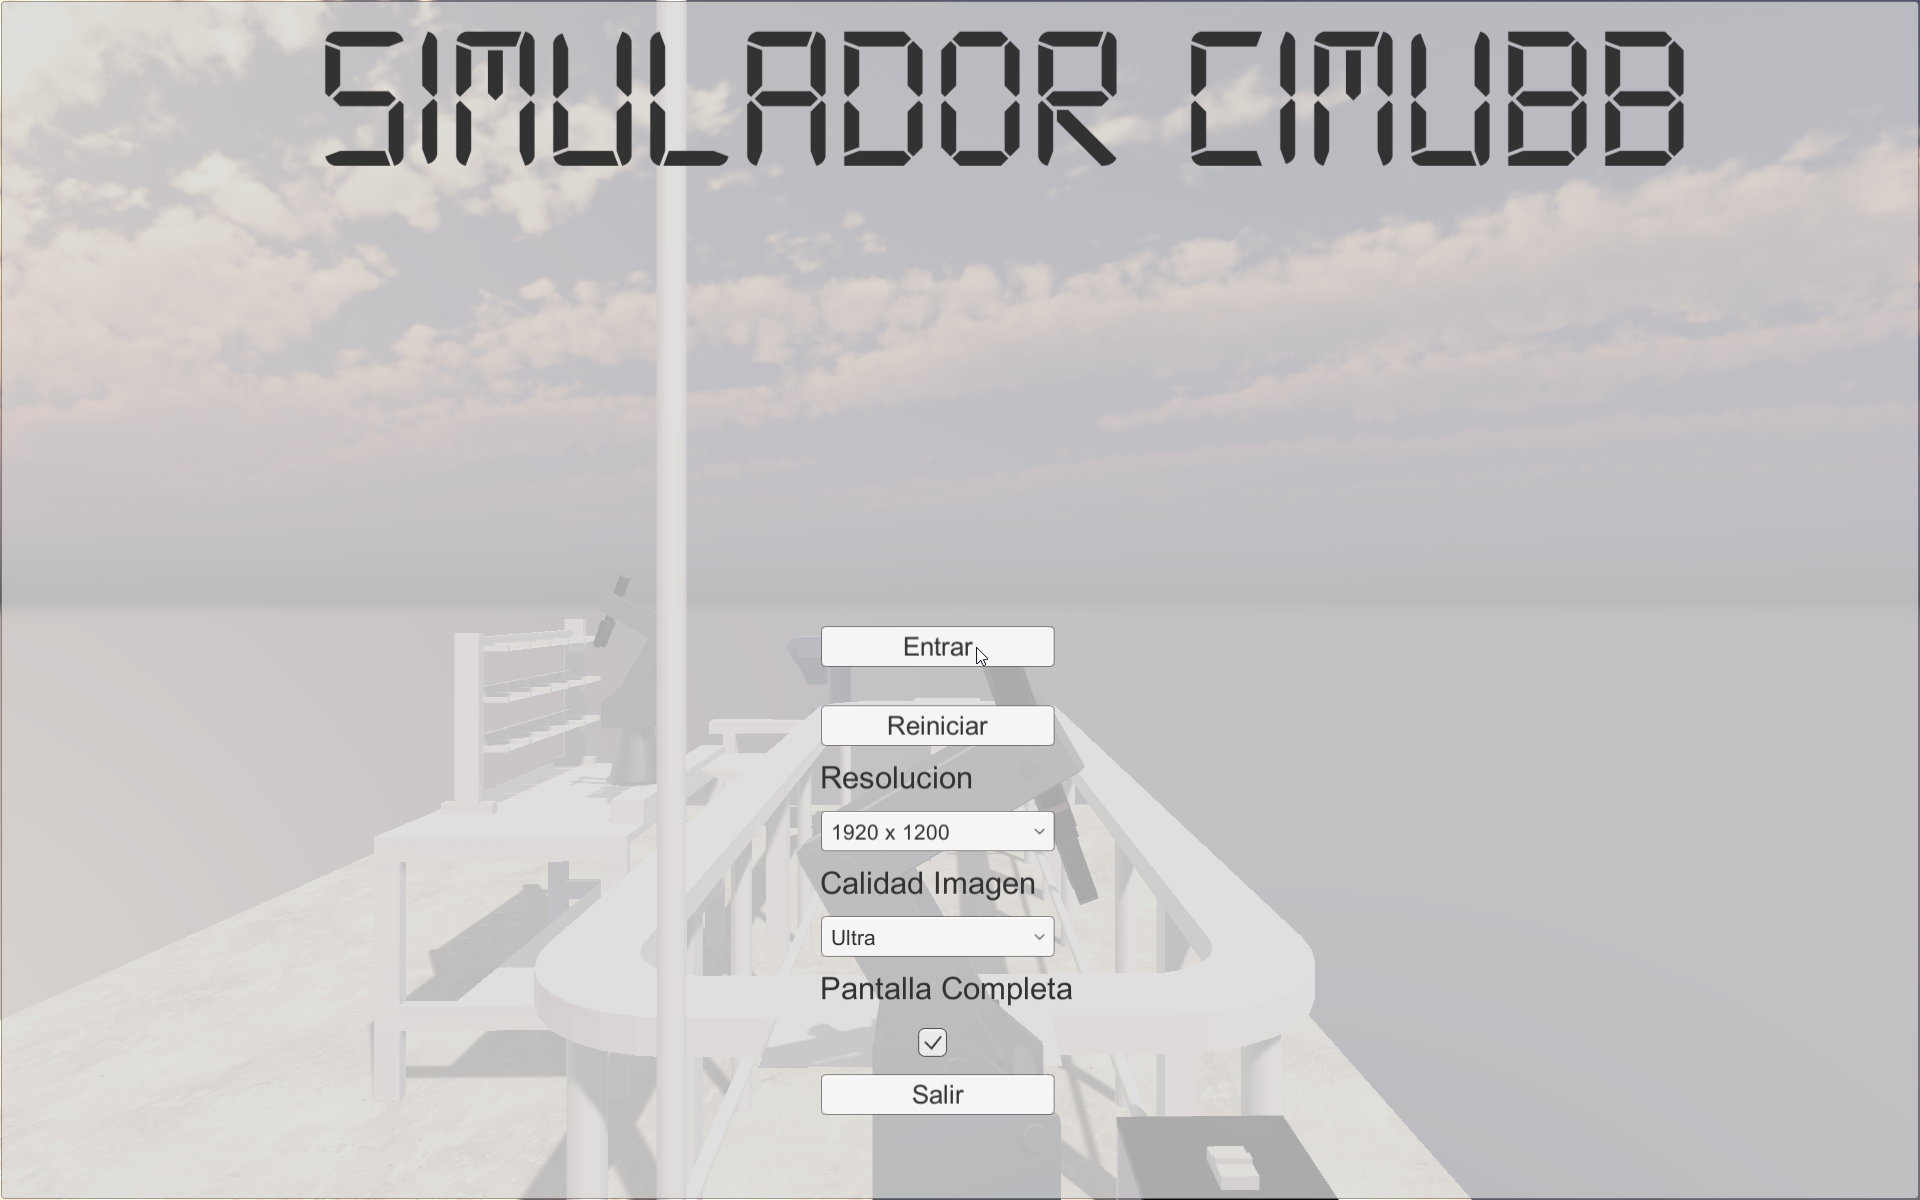
\includegraphics[width=13cm]{figures/TutorialWindows/tutorial (12).png}
    \caption{Parte 12 Tutorial Windows}
    \label{fig:tutowin12}
\end{figure}

\subsubsection*{Mac}

\begin{enumerate}[label=\arabic*.-]
    \item Utilizar la aplicación ''Unarchiver'' u otro programa de su preferencia para descomprimir archivos ZIP, o la línea de comandos.
    \item Descargar el archivo ZIP desde GitHub.
    \item En la línea de comandos: \verb|unzip nombre_del_archivo.zip|.
\end{enumerate}

\subsubsection*{Linux}

\begin{enumerate}[label=\arabic*.-]
    \item Verificar si el comando \verb|unzip| está instalado con: \verb|unzip --version|.
    \item Si no está instalado, instalarlo con el gestor de paquetes de tu distribución.
        \begin{itemize}
            \item Para Debian/Ubuntu: \verb|sudo apt-get install unzip|.
            \item Para Red Hat/Fedora: \verb|sudo yum install unzip|.
        \end{itemize}
    \item Descargar el archivo ZIP desde GitHub.
    \item Descomprimir el archivo ZIP con: \verb|unzip nombre_del_archivo.zip|.
\end{enumerate}

\subsubsection*{Mac}

\begin{itemize}
    \item Buscar el archivo ejecutable (con extensión .app o sin extensión) dentro de la carpeta descomprimida.
    \item Si es un archivo .app, hacer clic derecho y seleccionar ''Abrir'' para evitar problemas de seguridad.
    \item Si es un ejecutable, hacer doble clic para abrirlo.
\end{itemize}

\subsubsection*{Linux}

\begin{itemize}
    \item Abrir una terminal en la carpeta descomprimida.
    \item Verificar los permisos del archivo ejecutable con \verb|ls -l| y asegurarse de que sea ejecutable (\verb|chmod +x nombre_del_ejecutable| si es necesario).
    \item Ejecutar la aplicación desde la terminal con \verb|./nombre_del_ejecutable|.
\end{itemize}

Si bien algunas instrucciones pueden sonar como si el usuario necesitara tener un buen conocimiento sobre el equipo, la mayoría de los pasos implican funciones que normalmente uno realiza. Por ejemplo, enviar correos con archivos adjuntos comprimidos es una tarea común.